\documentclass[12pt,a4paper,oneside]{report}

% ---------------------------------------------------------------------------
% Encodage & langue
% ---------------------------------------------------------------------------
\usepackage[utf8]{inputenc}
\usepackage[T1]{fontenc}
\usepackage[french]{babel}
\usepackage{lmodern}

% ---------------------------------------------------------------------------
% Mise en page
% ---------------------------------------------------------------------------
\usepackage[a4paper,top=2cm,bottom=1.8cm,left=2.5cm,right=2.5cm]{geometry}
\usepackage{setspace}
\setstretch{1.15}
\usepackage{graphicx}
\usepackage{xcolor}
\usepackage{booktabs}
\usepackage{tabularx}
\usepackage{longtable}
\usepackage{array}
\usepackage{enumitem}
\usepackage{caption}
\usepackage{float}
\usepackage{fancyhdr}
\usepackage{titlesec}
\usepackage{eso-pic}
\usepackage{listings}
\usepackage[hidelinks]{hyperref}

% ---------------------------------------------------------------------------
% Couleurs (charte ESPRIT : rouge / gris)
% ---------------------------------------------------------------------------
\definecolor{espritred}{HTML}{CC0000}
\definecolor{espritgray}{HTML}{555555}
\definecolor{lightgray}{HTML}{F2F2F2}
\definecolor{codeback}{HTML}{F7F7F7}

% ---------------------------------------------------------------------------
% En-têtes / pieds de page
% ---------------------------------------------------------------------------
\pagestyle{fancy}
\fancyhf{}
\setlength{\headheight}{15pt}
\fancyhead[L]{\footnotesize\textcolor{espritgray}{Rapport de Stage d'Ingénieur}}
\fancyhead[R]{\footnotesize\textcolor{espritgray}{ESPRIT 2025--2026}}
\fancyfoot[C]{\thepage}
\renewcommand{\headrulewidth}{0.4pt}
\renewcommand{\footrulewidth}{0.2pt}

% Style des titres de chapitre
\titleformat{\chapter}[display]
  {\normalfont\huge\bfseries\color{espritred}}
  {\chaptertitlename\ \thechapter}{14pt}{\Huge}
\titlespacing*{\chapter}{0pt}{-10pt}{18pt}

% ---------------------------------------------------------------------------
% Style des listings de code
% ---------------------------------------------------------------------------
\lstset{
  backgroundcolor=\color{codeback},
  basicstyle=\ttfamily\scriptsize,
  keywordstyle=\color{espritred}\bfseries,
  commentstyle=\color{espritgray}\itshape,
  stringstyle=\color{teal},
  breaklines=true,
  showstringspaces=false,
  frame=single,
  rulecolor=\color{lightgray},
  numbers=left,
  numberstyle=\tiny\color{espritgray},
  captionpos=b,
  tabsize=2,
}

\newcommand{\sut}{\textit{LaRuche}}

% ===========================================================================
\begin{document}

% ---------------------------------------------------------------------------
% PAGE DE GARDE (image fournie)
% ---------------------------------------------------------------------------
\begin{titlepage}
\thispagestyle{empty}
\newgeometry{margin=0cm}
\AddToShipoutPictureBG*{%
  \AtPageCenter{%
    \makebox(0,0){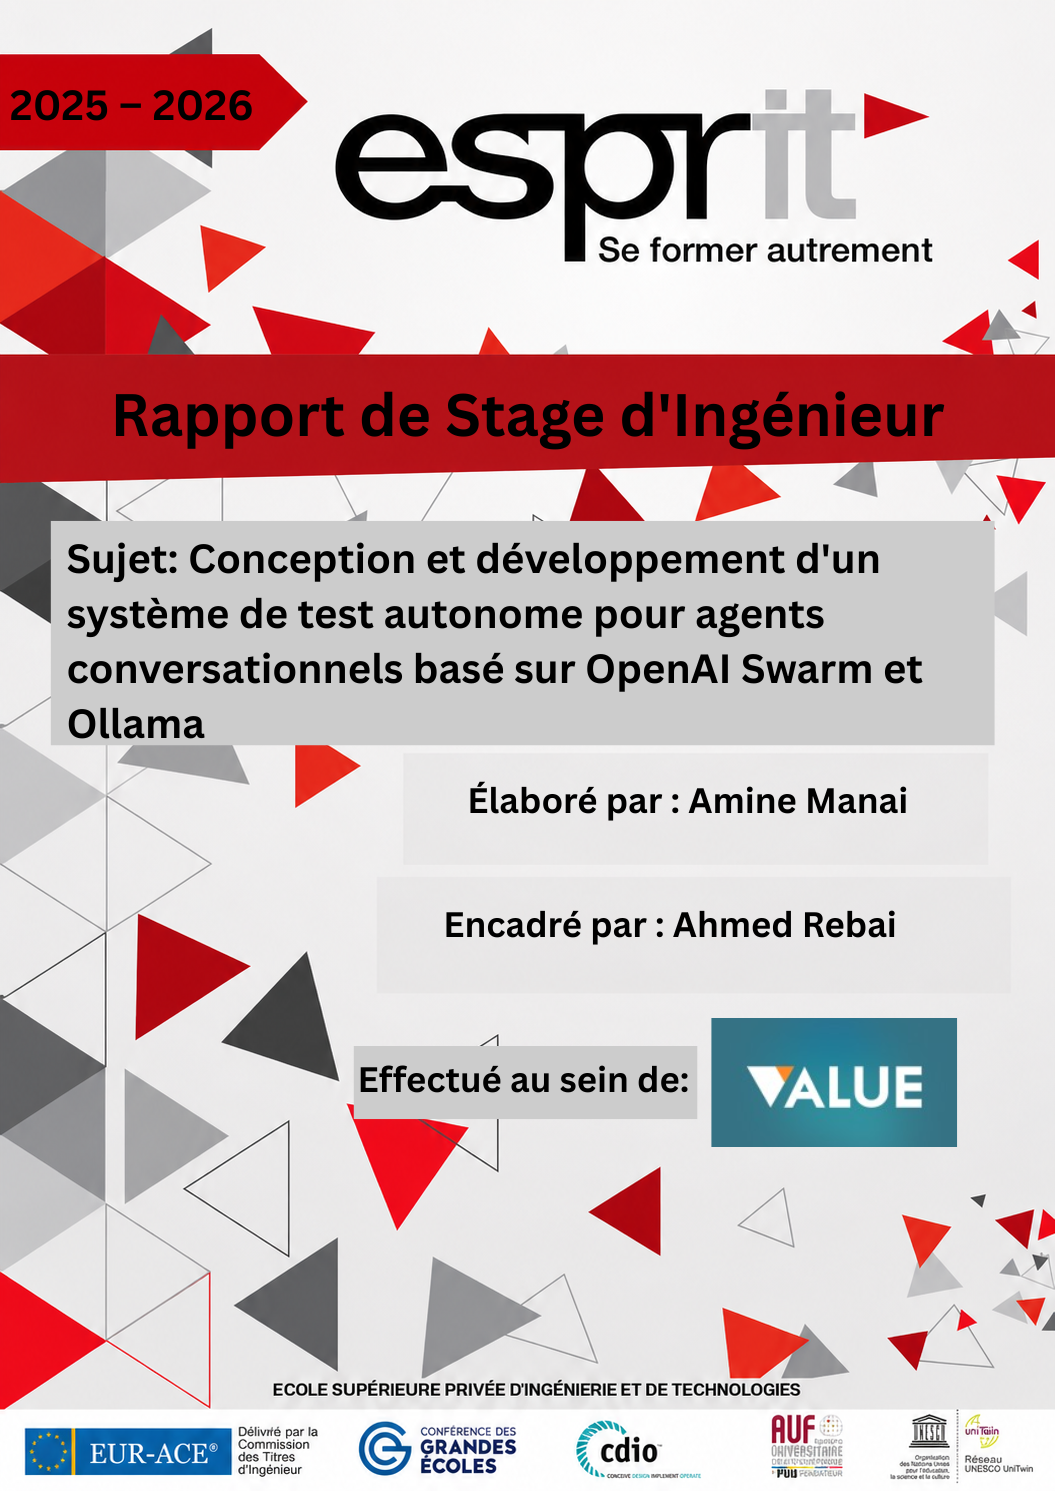
\includegraphics[width=\paperwidth,height=\paperheight,keepaspectratio]{page_de_garde.png}}%
  }%
}
\mbox{}
\restoregeometry
\end{titlepage}

% ---------------------------------------------------------------------------
% Pages liminaires
% ---------------------------------------------------------------------------
\pagenumbering{roman}

% --- Remerciements ---
\chapter*{Remerciements}
\addcontentsline{toc}{chapter}{Remerciements}
\markboth{Remerciements}{Remerciements}

Au terme de ce stage d'ingénieur, je tiens à exprimer ma profonde gratitude à
toutes les personnes qui ont contribué, de près ou de loin, à la réussite de cette
expérience.

Je remercie tout d'abord la société \textbf{Value} de m'avoir accueilli et de
m'avoir confié un sujet aussi stimulant, au croisement de l'intelligence
artificielle générative et de l'assurance qualité logicielle.

J'adresse mes remerciements les plus sincères à mon encadrant professionnel,
\textbf{Monsieur Ahmed Rebai}, pour sa disponibilité, ses conseils avisés et la
confiance qu'il m'a accordée tout au long de ce stage. Son expertise et son
accompagnement ont été déterminants dans l'orientation et la concrétisation de ce
travail.

Je remercie également le corps enseignant et l'administration de l'\textbf{École
Supérieure Privée d'Ingénierie et de Technologies (ESPRIT)} pour la qualité de la
formation dispensée, qui m'a permis d'aborder ce projet avec les compétences
nécessaires.

Enfin, je tiens à exprimer ma reconnaissance à ma famille et à mes amis pour leur
soutien constant et leurs encouragements.

% --- Résumé ---
\chapter*{Résumé}
\addcontentsline{toc}{chapter}{Résumé}
\markboth{Résumé}{Résumé}

Ce rapport présente le travail réalisé durant un stage d'ingénieur de deux mois au
sein de la société \textbf{Value}. Le projet consiste à concevoir et développer un
\textbf{système de test autonome} pour les agents conversationnels, fondé sur le
framework multi-agents \textbf{OpenAI Swarm} et sur des petits modèles de langage
(\textit{Small Language Models}, SLM) exécutés localement via \textbf{Ollama}.

Le système, baptisé \textbf{QA-Swarm}, automatise l'ensemble du cycle de test d'un
agent conversationnel financier : génération de scénarios, exécution multi-canal
(API REST, Web, Mobile), évaluation de la qualité des réponses (pertinence,
exactitude, cohérence, hallucination), production de rapports interactifs et, enfin,
\textbf{détection de régressions} entre deux versions de l'agent testé. Une console
d'administration (\textit{backoffice}) permet de piloter les campagnes de test et de
visualiser les tableaux de bord.

La principale contribution de ce travail est une chaîne de test entièrement
orchestrée par des agents autonomes (\textit{Generator} $\rightarrow$
\textit{Executor} $\rightarrow$ \textit{Evaluator} $\rightarrow$ \textit{Reporter}
$\rightarrow$ \textit{FixPlanner}), capable de juger automatiquement la qualité d'un
agent conversationnel et de signaler toute dégradation introduite par une nouvelle
version.

\vspace{0.3cm}
\noindent\textbf{Mots-clés :} test autonome, agents conversationnels, OpenAI Swarm,
SLM, Ollama, détection de régression, hallucination, assurance qualité, LLM-as-a-judge.

\vspace{0.5cm}
\noindent\textbf{\large Abstract}
\vspace{0.15cm}


This report describes a two-month engineering internship carried out at
\textbf{Value}. The project consists in designing and building an
\textbf{autonomous testing system} for conversational agents, based on the
\textbf{OpenAI Swarm} multi-agent framework and on \textbf{Small Language Models}
running locally through \textbf{Ollama}. The resulting system, \textbf{QA-Swarm},
automates the full testing lifecycle of a financial conversational agent: scenario
generation, multi-channel execution (REST API, Web, Mobile), answer-quality
evaluation, interactive reporting, and \textbf{regression detection} between two
versions of the agent under test, all driven by an autonomous agent handoff chain.

\vspace{0.2cm}
\noindent\textbf{Keywords:} autonomous testing, conversational agents, OpenAI Swarm,
SLM, Ollama, regression detection, hallucination, quality assurance, LLM-as-a-judge.

% --- Table des matières ---
\tableofcontents

% ---------------------------------------------------------------------------
% Corps du rapport
% ---------------------------------------------------------------------------
\clearpage
\pagenumbering{arabic}

% ===========================================================================
\chapter*{Introduction générale}
\addcontentsline{toc}{chapter}{Introduction générale}
\markboth{Introduction générale}{Introduction générale}

L'essor des grands modèles de langage (\textit{Large Language Models}, LLM) a fait
des agents conversationnels une brique centrale des produits numériques modernes :
assistants, chatbots de support, conseillers virtuels. Dans le domaine financier en
particulier, un agent conversationnel peut répondre à des questions sur un
portefeuille, calculer des indicateurs de performance ou produire des synthèses.
Cette puissance s'accompagne toutefois d'un risque majeur : l'\textbf{imprévisibilité}.
Contrairement à un logiciel déterministe, un agent fondé sur un modèle de langage peut
fournir des réponses différentes à la même question, inventer des faits
(\textit{hallucinations}), ou voir sa qualité se dégrader silencieusement lorsqu'on
modifie son \textit{prompt}, son modèle sous-jacent ou son code de routage.

Les méthodes de test traditionnelles, fondées sur des assertions exactes
(\textit{entrée} $\rightarrow$ \textit{sortie attendue}), sont mal adaptées à ce type
de système : il n'existe pas une seule « bonne » réponse, mais un espace de réponses
acceptables. Tester un agent conversationnel impose donc d'\textbf{évaluer la qualité
sémantique} d'une réponse plutôt que sa stricte égalité à une référence, et de le
faire à grande échelle, de manière reproductible, et sur tous les canaux par lesquels
l'utilisateur accède au service.

C'est dans ce contexte que s'inscrit le présent stage. L'objectif est de concevoir un
\textbf{système de test autonome} capable de tester de bout en bout un agent
conversationnel financier, sur ses trois surfaces d'accès (API REST, application Web,
application Mobile), d'évaluer automatiquement la qualité de ses réponses, et surtout
de \textbf{détecter les régressions} entre deux versions successives de l'agent.

Le système développé, \textbf{QA-Swarm}, repose sur le framework multi-agents
\textbf{OpenAI Swarm} et sur des petits modèles de langage exécutés localement via
\textbf{Ollama}, ce qui garantit confidentialité et coût nul d'inférence. L'agent
conversationnel testé, nommé \sut{}, est une plateforme de gestion de patrimoine
construite comme un maillage (\textit{mesh}) d'agents spécialisés ; il joue le rôle de
\textbf{système sous test} (\textit{System Under Test}, SUT).

Ce rapport est organisé en cinq chapitres. Le \textbf{premier} présente le contexte
général du projet : l'entreprise d'accueil, la problématique et la méthodologie de
travail. Le \textbf{deuxième} dresse une étude de l'état de l'art du test des agents
conversationnels et des technologies retenues. Le \textbf{troisième} formalise
l'analyse et la spécification des besoins. Le \textbf{quatrième} détaille la
conception de l'architecture du système. Le \textbf{cinquième} décrit la réalisation
et les résultats obtenus. Une conclusion générale et des perspectives clôturent le
document.

% ===========================================================================
\chapter{Contexte général du projet}

\section{Introduction}
Ce premier chapitre situe le projet dans son cadre. Il présente l'organisme
d'accueil, expose la problématique à l'origine du sujet, définit les objectifs du
stage et décrit la méthodologie de travail adoptée.

\section{Organisme d'accueil}
Ce stage s'est déroulé au sein de la société \textbf{Value}, une entreprise active
dans le domaine de l'ingénierie logicielle et de l'intelligence artificielle. Value
accompagne ses clients dans la conception de solutions logicielles innovantes, avec un
intérêt marqué pour les technologies d'IA générative et leur industrialisation. Dans
ce cadre, l'entreprise s'intéresse aux enjeux de fiabilité et de qualité des systèmes
fondés sur des modèles de langage, qui constituent le cœur du présent projet.

\section{Cadre du stage}
Le stage, d'une durée de \textbf{deux mois} (du 12 juin 2026 au 12 août 2026),
s'inscrit dans le cursus d'ingénieur de l'ESPRIT. Il correspond à un stage
d'ingénieur visant à mettre en application les compétences acquises en
développement logiciel, en intelligence artificielle et en génie logiciel, dans un
contexte professionnel réel.

\section{Étude de l'existant et problématique}

\subsection{Le système à tester}
L'objet du test est un agent conversationnel financier, \sut{}, conçu comme un
\textbf{maillage d'agents} (\textit{agentic mesh}). Une requête utilisateur est reçue
par un \textbf{orchestrateur} qui la route, selon son intention, vers un ou plusieurs
agents spécialisés (financier, marché, documents, action, qualité), puis agrège les
réponses et les renvoie en flux continu (\textit{streaming}). Cet agent est accessible
par trois canaux distincts : une \textbf{API REST}, une \textbf{application Web} et une
\textbf{application Mobile}.

\subsection{Problématique}
La nature non déterministe de cet agent soulève plusieurs difficultés que les
approches de test classiques ne savent pas traiter :

\begin{itemize}[leftmargin=*]
  \item \textbf{Absence de sortie unique de référence} : à une même question peuvent
  correspondre plusieurs réponses correctes formulées différemment. Une comparaison
  exacte n'a donc pas de sens.
  \item \textbf{Risque d'hallucination} : l'agent peut inventer des chiffres ou des
  faits non fondés, ce qui est particulièrement grave dans un contexte financier.
  \item \textbf{Régressions silencieuses} : une modification du \textit{prompt}, du
  modèle ou du code de routage peut dégrader la qualité sans provoquer d'erreur
  visible.
  \item \textbf{Multiplicité des canaux} : le même agent doit se comporter de manière
  cohérente sur l'API, le Web et le Mobile.
  \item \textbf{Robustesse} : l'agent doit résister aux entrées limites (vides, très
  longues) et aux attaques (injection de \textit{prompt}, XSS, questions hors domaine).
\end{itemize}

La question centrale du stage est donc la suivante : \emph{comment tester de manière
automatique, reproductible et multi-canal un agent conversationnel, en évaluant la
qualité sémantique de ses réponses et en détectant toute régression entre deux
versions ?}

\section{Objectifs du projet}
Pour répondre à cette problématique, le projet vise les objectifs suivants :
\begin{enumerate}[leftmargin=*]
  \item Concevoir une \textbf{chaîne de test autonome} orchestrée par des agents
  (génération, exécution, évaluation, rapport, planification de correctifs).
  \item Couvrir les \textbf{trois canaux} d'accès : API REST, Web et Mobile.
  \item Évaluer automatiquement la qualité des réponses selon des critères
  sémantiques (pertinence, exactitude, cohérence) et détecter les hallucinations.
  \item Produire des \textbf{rapports} lisibles et des tableaux de bord interactifs.
  \item Implémenter la \textbf{détection de régression} entre deux versions de
  l'agent — critère de succès central du projet.
  \item Offrir une \textbf{console d'administration} pour piloter les campagnes.
\end{enumerate}

\section{Méthodologie de travail}
Le projet a été conduit selon une démarche \textbf{itérative et incrémentale},
inspirée des méthodes agiles. Le travail a été découpé en phases successives, chacune
livrant un incrément fonctionnel et vérifiable : mise en place de l'infrastructure et
du lien Swarm/Ollama, puis canal API, puis canaux Web et Mobile, puis métriques et
tableaux de bord, puis détection de régression, et enfin console d'administration. Le
code est versionné avec \textbf{Git} et chaque composant est accompagné de tests
automatisés.

\section{Conclusion}
Ce chapitre a posé le cadre du stage et formulé la problématique : tester de façon
autonome et multi-canal un agent conversationnel non déterministe. Le chapitre suivant
étudie l'état de l'art et justifie les choix technologiques.

% ===========================================================================
\chapter{État de l'art et étude technologique}

\section{Introduction}
Ce chapitre présente les concepts et technologies sur lesquels repose le projet : la
spécificité du test des agents conversationnels, les petits modèles de langage, le
framework OpenAI Swarm, les outils de test multi-canal et les techniques d'évaluation
de la qualité.

\section{Le test des agents conversationnels}
Tester un système fondé sur un LLM diffère fondamentalement du test logiciel
classique. On distingue plusieurs niveaux :
\begin{itemize}[leftmargin=*]
  \item \textbf{Test fonctionnel} : vérifier que l'agent répond à l'intention de
  l'utilisateur.
  \item \textbf{Test de qualité sémantique} : mesurer la pertinence, l'exactitude et
  la cohérence de la réponse plutôt que son égalité exacte à une référence.
  \item \textbf{Test de robustesse} : éprouver l'agent sur des entrées limites et des
  prompts adverses.
  \item \textbf{Test de non-régression} : garantir qu'une nouvelle version ne dégrade
  pas le comportement existant.
\end{itemize}
La difficulté majeure réside dans l'\textbf{évaluation automatique} : faute de sortie
de référence unique, on recourt de plus en plus au paradigme \textbf{LLM-as-a-judge},
où un modèle de langage joue le rôle de juge et note la réponse selon une grille de
critères.

\section{Les petits modèles de langage (SLM) et Ollama}
Les \textbf{Small Language Models} (SLM) sont des modèles de langage de taille réduite
(quelques milliards de paramètres) qui peuvent s'exécuter localement sur du matériel
grand public. Ils offrent plusieurs avantages décisifs pour un système de test :
\textbf{confidentialité} (aucune donnée ne quitte la machine), \textbf{coût nul}
d'inférence et \textbf{reproductibilité}.

\textbf{Ollama} est un environnement d'exécution qui permet de télécharger et de servir
des SLM localement en exposant une API compatible avec celle d'OpenAI. Le projet
utilise principalement le modèle \texttt{qwen2.5:3b}, retenu pour sa fiabilité dans
l'appel d'outils (\textit{tool-calling}), indispensable aux passages de relais
(\textit{handoffs}) du framework Swarm, et pour sa compacité (il tient intégralement
dans 4~Go de mémoire vidéo).

\section{OpenAI Swarm}
\textbf{OpenAI Swarm} est un framework expérimental d'orchestration multi-agents. Il
repose sur deux primitives simples :
\begin{itemize}[leftmargin=*]
  \item les \textbf{Agents}, définis par un nom, un modèle, des instructions
  (\textit{system prompt}) et un ensemble de fonctions ;
  \item les \textbf{handoffs}, mécanisme par lequel un agent passe le relais à un autre
  en retournant simplement une référence vers cet agent.
\end{itemize}
Cette légèreté en fait un candidat idéal pour modéliser une chaîne de test où chaque
étape (génération, exécution, évaluation, rapport) est prise en charge par un agent
spécialisé, selon le principe « \textbf{un agent = un SLM} ». Swarm communiquant via
une API compatible OpenAI, il se branche directement sur Ollama.

\section{Outils de test multi-canal}
\subsection{API REST}
Le test de l'API se fait par requêtes HTTP directes. Le client \textbf{httpx} (Python)
permet d'envoyer des requêtes et de consommer un flux \textbf{Server-Sent Events}
(SSE), protocole utilisé par l'agent pour renvoyer ses réponses jeton par jeton.

\subsection{Playwright (Web)}
\textbf{Playwright} est un framework moderne d'automatisation de navigateur. Plus
rapide et plus fiable que l'historique Selenium grâce à son attente automatique des
éléments, il pilote un navigateur \textit{Chromium} pour simuler un utilisateur réel
sur l'application Web.

\subsection{Appium (Mobile)}
\textbf{Appium} est le standard de l'automatisation des applications mobiles. Via le
pilote \textit{UiAutomator2}, il contrôle l'application sur un émulateur Android et y
reproduit les interactions de l'utilisateur.

\section{Techniques d'évaluation de la qualité textuelle}
Outre le jugement par LLM, le projet emploie des métriques classiques de comparaison
de texte :
\begin{itemize}[leftmargin=*]
  \item \textbf{BLEU} (via \texttt{sacrebleu}) et \textbf{ROUGE-L} (via
  \texttt{rouge-score}), qui mesurent le recouvrement lexical entre la réponse obtenue
  et la réponse attendue ;
  \item la \textbf{similarité de séquence} (\texttt{difflib}), utilisée pour mesurer la
  \textbf{divergence} entre les réponses des canaux Web et Mobile.
\end{itemize}

\section{Conclusion}
L'étude technologique a montré la pertinence d'une approche fondée sur des agents
autonomes (Swarm) et des SLM locaux (Ollama), complétée par des outils de test
éprouvés (httpx, Playwright, Appium) et des techniques d'évaluation sémantique. Le
chapitre suivant formalise les besoins du système.

% ===========================================================================
\chapter{Analyse et spécification des besoins}

\section{Introduction}
Ce chapitre identifie les acteurs du système, recense les besoins fonctionnels et non
fonctionnels, et précise le périmètre du système sous test.

\section{Identification des acteurs}
\begin{itemize}[leftmargin=*]
  \item \textbf{L'ingénieur QA / développeur} : déclenche les campagnes de test,
  consulte les rapports et les plans de correctifs, compare deux versions de l'agent.
  \item \textbf{Le système d'intégration continue (CI)} : exécute automatiquement un
  test de fumée (\textit{smoke test}) à chaque modification, afin de bloquer toute
  régression bloquante avant fusion.
  \item \textbf{L'agent sous test (\sut{})} : acteur secondaire, sollicité par le
  système de test sur ses trois canaux.
\end{itemize}

\section{Besoins fonctionnels}
Le système doit permettre de :
\begin{enumerate}[leftmargin=*]
  \item \textbf{Générer} un corpus de scénarios de test (nominaux, limites, adverses),
  versionné en JSON, et en synthétiser de nouveaux à partir d'une spécification.
  \item \textbf{Exécuter} chaque scénario sur les canaux ciblés (API, Web, Mobile).
  \item \textbf{Évaluer} la réponse selon la pertinence, l'exactitude, la cohérence et
  la présence d'hallucinations, puis rendre un verdict PASS/FAIL.
  \item \textbf{Mesurer} la latence, le temps de première réponse, la disponibilité et
  la divergence entre canaux.
  \item \textbf{Produire} un rapport Markdown et un tableau de bord HTML interactif.
  \item \textbf{Détecter les régressions} entre deux exécutions (passages PASS$\to$FAIL,
  chutes de score, hausses de latence).
  \item \textbf{Proposer} des plans de correctifs non destructifs pour les échecs.
  \item \textbf{Piloter} l'ensemble depuis une console d'administration Web.
\end{enumerate}

\section{Besoins non fonctionnels}
\begin{itemize}[leftmargin=*]
  \item \textbf{Confidentialité} : l'inférence doit être 100\,\% locale (aucune donnée
  envoyée à un service tiers).
  \item \textbf{Reproductibilité} : les scénarios sont versionnés et les exécutions
  horodatées et persistées.
  \item \textbf{Modularité} : chaque agent et chaque canal doit être indépendant et
  remplaçable.
  \item \textbf{Sécurité} : le planificateur de correctifs ne doit jamais modifier le
  code (principe de non-destruction).
  \item \textbf{Robustesse} : un échec sur un canal ne doit pas interrompre la
  campagne.
  \item \textbf{Configurabilité} : URLs, modèles et seuils sont paramétrables par
  variables d'environnement.
\end{itemize}

\section{Le système sous test (SUT)}
L'agent \sut{} est composé de sept services indépendants, présentés au
tableau~\ref{tab:services}. C'est sur cet ensemble que s'exerce le système de test, en
priorité via le point d'entrée \texttt{POST /api/chat} de l'orchestrateur.

\begin{table}[H]
\centering
\caption{Services composant l'agent sous test (\sut{}).}
\label{tab:services}
\renewcommand{\arraystretch}{1.3}
\begin{tabularx}{\textwidth}{@{}l l X@{}}
\toprule
\textbf{Service} & \textbf{Port} & \textbf{Rôle} \\
\midrule
Orchestrateur & 8000 & Routage des requêtes, agrégation, flux SSE \\
Agent financier & 8001 & Indicateurs de portefeuille (AUM, TWR, IRR, Sharpe) \\
Agent marché & 8002 & Données de marché et cotations \\
Agent documents & 8003 & Recherche documentaire (RAG) \\
Agent action & 8004 & Actions (envoi de courriel, messages) \\
Agent QA & 8005 & Génération et exécution de tests internes \\
Service vocal & 8006 & Transcription et synthèse vocale \\
\bottomrule
\end{tabularx}
\end{table}

Les figures~\ref{fig:sut-dashboard} et \ref{fig:sut-chat} illustrent l'interface
utilisateur du SUT : le tableau de bord de portefeuille et l'assistant conversationnel.

\begin{figure}[H]
\centering
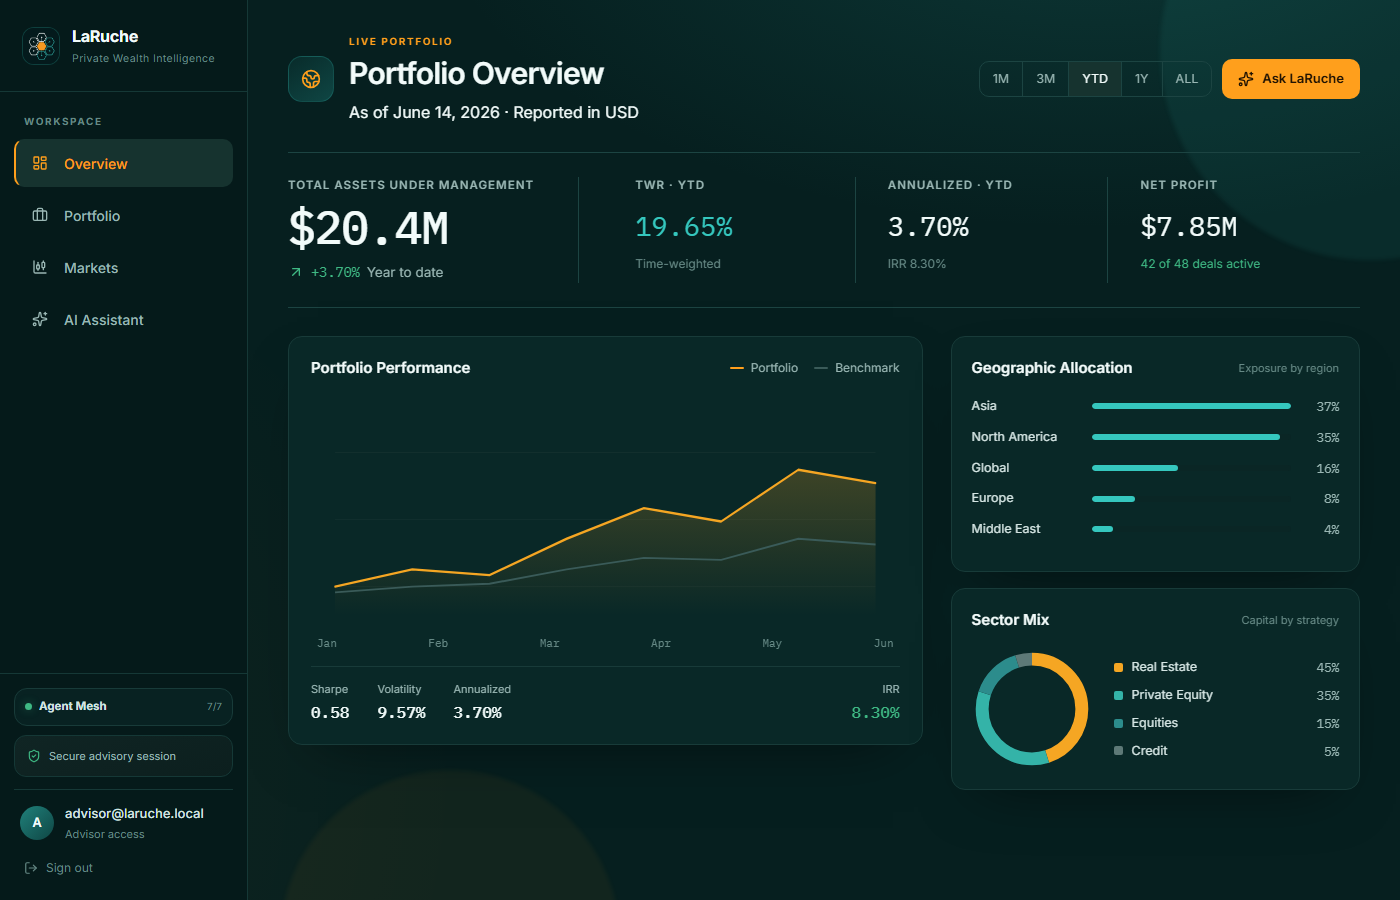
\includegraphics[width=0.82\textwidth]{screenshot_dashboard.png}
\caption{Tableau de bord du SUT \sut{} — vue portefeuille avec indicateurs financiers.}
\label{fig:sut-dashboard}
\end{figure}

\begin{figure}[H]
\centering
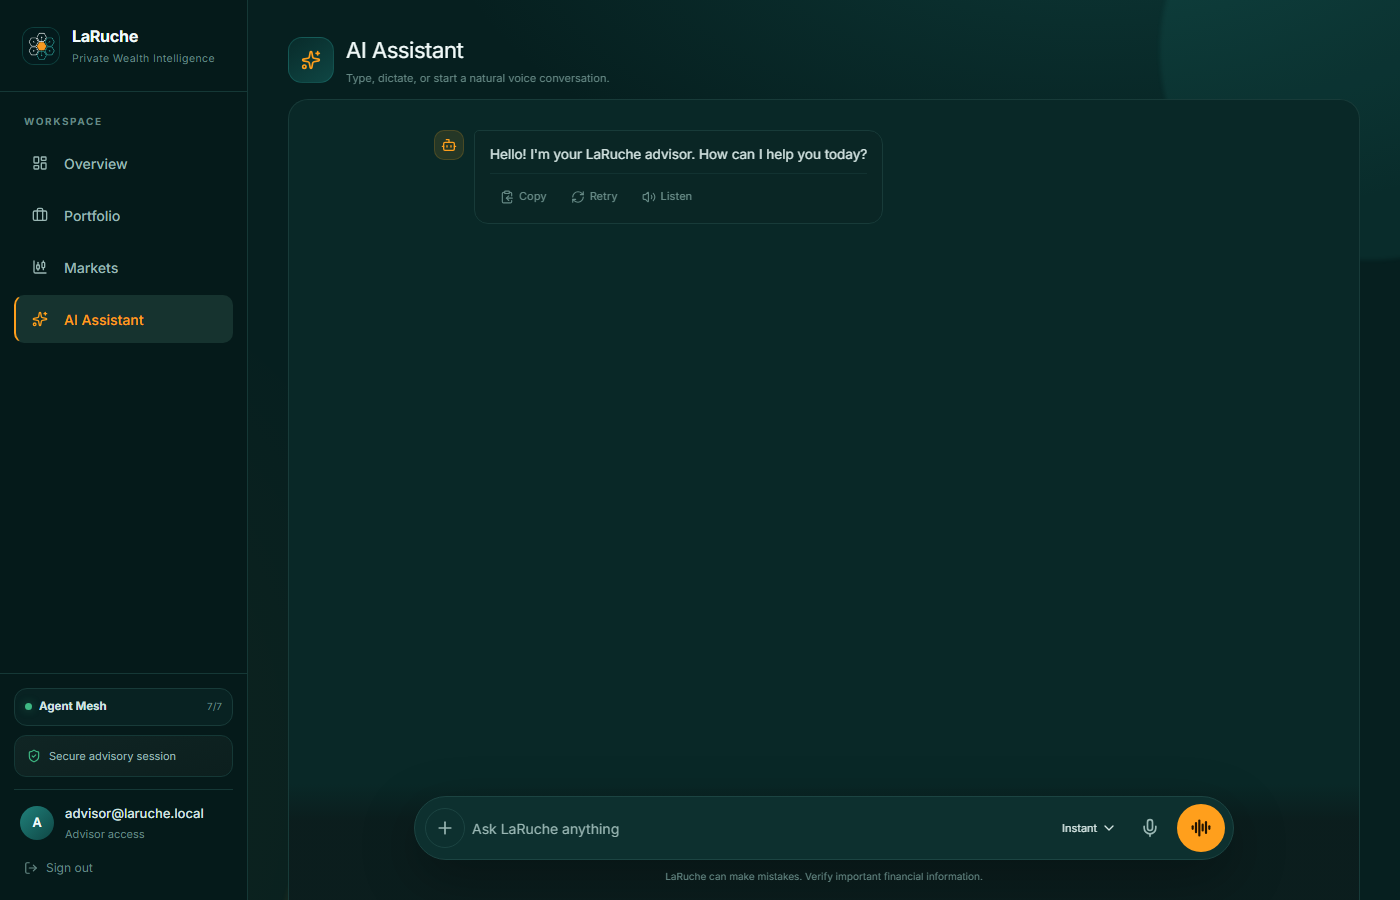
\includegraphics[width=0.82\textwidth]{screenshot_chat.png}
\caption{Interface de l'assistant conversationnel du SUT (Agent Mesh 7/7).}
\label{fig:sut-chat}
\end{figure}

\section{Conclusion}
Les besoins étant clarifiés et le périmètre du SUT défini, le chapitre suivant en
présente la conception détaillée.

% ===========================================================================
\chapter{Conception du système}

\section{Introduction}
Ce chapitre décrit l'architecture globale de QA-Swarm, le rôle de chaque agent, la
conception des canaux, le mécanisme de scoring, la détection de régression et le modèle
de données.

\section{Architecture globale}
QA-Swarm est organisé comme une \textbf{chaîne d'agents autonomes} reliés par des
passages de relais. Le flux est le suivant :

\begin{center}
\fbox{\textbf{Generator} $\rightarrow$ \textbf{Executor} $\rightarrow$ \textbf{Evaluator}
$\rightarrow$ \textbf{Reporter} $\rightarrow$ \textbf{FixPlanner}}
\end{center}

Chaque agent est un agent Swarm doté de son propre SLM (servi par Ollama) et d'un rôle
unique. Le tableau~\ref{tab:agents} récapitule ces rôles.

\begin{table}[H]
\centering
\caption{Les agents de la chaîne QA-Swarm.}
\label{tab:agents}
\renewcommand{\arraystretch}{1.3}
\begin{tabularx}{\textwidth}{@{}l X l@{}}
\toprule
\textbf{Agent} & \textbf{Rôle} & \textbf{Modèle} \\
\midrule
Generator & Charge le corpus JSON ou synthétise des scénarios & qwen2.5:3b \\
Executor & Dispatche chaque cas vers API, Web ou Mobile & qwen2.5:3b \\
Evaluator & Note pertinence, exactitude, cohérence, hallucination & qwen2.5:3b \\
Reporter & Produit les rapports Markdown et HTML (Plotly) & qwen2.5:3b \\
FixPlanner & Classe les échecs et écrit des plans de correctifs sûrs & heuristiques / qwen2.5:3b \\
\bottomrule
\end{tabularx}
\end{table}

\section{Conception des canaux de test}
Trois canaux partagent une même interface (\texttt{ChannelResult}) mais diffèrent dans
leur exécution :
\begin{itemize}[leftmargin=*]
  \item \textbf{Canal API} : envoi direct d'une requête HTTP sur \texttt{/api/chat},
  consommation du flux SSE, mesure de la latence et du temps de première réponse
  (\textit{TTFT}). Pur \texttt{httpx}, sans interface ni LLM.
  \item \textbf{Canal Web} : selon la philosophie « \textit{code-based} », le SLM de
  l'\textit{Executor} \textbf{génère un script Playwright complet} pour le scénario.
  Ce script est validé par \texttt{ast.parse} puis exécuté dans un \textbf{bac à sable}
  (sous-processus avec délai limite). Un script de repli éprouvé est utilisé si la
  génération échoue.
  \item \textbf{Canal Mobile} : même principe \textit{code-based} avec un script Appium
  ciblant l'émulateur Android.
\end{itemize}

\section{Conception du scoring}
L'évaluation combine un \textbf{juge LLM} et des \textbf{règles déterministes}. Les
règles d'échec \textbf{bloquantes} sont appliquées en premier, sans appel au modèle :
\begin{itemize}[leftmargin=*]
  \item dépassement du délai (\textit{timeout}, 30~s) ;
  \item plantage ou erreur serveur (5xx) ;
  \item réponse vide ;
  \item hallucination détectée.
\end{itemize}
En l'absence de ces conditions, le juge LLM note la réponse sur trois axes (pertinence,
exactitude, cohérence) de 1 à 5 et signale toute hallucination. Le verdict final est
\textbf{calculé de façon déterministe} : une hallucination entraîne un échec ; sinon, la
réponse passe si la moyenne des trois scores atteint le seuil de~3,0. Ce choix
— laisser le LLM noter mais décider la règle en dur — est plus fiable que de confier
l'application de la règle à un modèle de 3 milliards de paramètres.

\section{Conception de la détection de régression}
La détection de régression est le \textbf{critère de succès} du projet. Elle compare
deux exécutions complètes (\texttt{RunReport}), une \textit{baseline} et une
\textit{candidate}, appariées par intention et par canal. Trois types de régression
sont signalés :
\begin{itemize}[leftmargin=*]
  \item \textbf{Bascule PASS$\to$FAIL} : un scénario qui passait échoue désormais ;
  \item \textbf{Chute de score} : baisse de la moyenne d'au moins 0,5 point ;
  \item \textbf{Pic de latence} : hausse de la latence d'au moins 50\,\%.
\end{itemize}

\section{Conception du planificateur de correctifs}
Le \textbf{FixPlanner} est volontairement \textbf{non destructif} : il n'écrit jamais
de code. Pour chaque échec, il produit un \textbf{triage} (catégorie, sévérité,
confiance, propriétaire probable, preuves) et un \textbf{plan de correctif} (hypothèse
de cause racine, fichiers probables, étapes, commandes de vérification, notes de retour
arrière). Tout plan porte les drapeaux \texttt{auto\_apply=false} et
\texttt{human\_approval\_required=true}.

\section{Modèle de données}
Les structures de données, validées par \textbf{Pydantic}, garantissent la cohérence de
toute la chaîne. Les principales entités sont résumées au tableau~\ref{tab:models}.

\begin{table}[H]
\centering
\caption{Principales structures de données.}
\label{tab:models}
\renewcommand{\arraystretch}{1.3}
\begin{tabularx}{\textwidth}{@{}l X@{}}
\toprule
\textbf{Entité} & \textbf{Description} \\
\midrule
\texttt{TestCase} & Un scénario : id, intention, type, entrée, attendu, canaux \\
\texttt{ChannelResult} & Résultat brut sur un canal : réponse, statut, latence, TTFT, drapeaux \\
\texttt{Score} & Notes pertinence/exactitude/cohérence, hallucination, verdict \\
\texttt{ScenarioResult} & Un cas + ses résultats et scores par canal + divergence \\
\texttt{RunReport} & Une exécution complète (unité comparée pour la régression) \\
\texttt{FailureAnalysis} & Triage + plan de correctif d'un échec \\
\bottomrule
\end{tabularx}
\end{table}

\section{Conclusion}
La conception ayant fixé l'architecture, les agents, les canaux et les mécanismes
d'évaluation, le chapitre suivant en présente la réalisation concrète.

% ===========================================================================
\chapter{Réalisation}

\section{Introduction}
Ce chapitre présente l'environnement technique, des extraits significatifs de
l'implémentation, le corpus de test, la console d'administration et les résultats
obtenus.

\section{Environnement de travail}
\subsection{Environnement matériel}
Le développement a été mené sur une station de travail équipée d'un processeur
multi-cœurs, de 16~Go de mémoire vive et d'une carte graphique disposant de 4~Go de
mémoire vidéo, suffisante pour exécuter le modèle \texttt{qwen2.5:3b} via Ollama.

\subsection{Environnement logiciel}
Le tableau~\ref{tab:tools} récapitule les principaux outils et technologies utilisés.

\begin{table}[H]
\centering
\caption{Environnement logiciel du projet.}
\label{tab:tools}
\renewcommand{\arraystretch}{1.3}
\begin{tabularx}{\textwidth}{@{}l X@{}}
\toprule
\textbf{Catégorie} & \textbf{Outils} \\
\midrule
Langage & Python 3.12 \\
Orchestration d'agents & OpenAI Swarm \\
Exécution des modèles & Ollama (\texttt{qwen2.5:3b}) \\
Tests de canaux & httpx (API), Playwright (Web), Appium (Mobile) \\
Validation de données & Pydantic \\
Métriques NLP & sacrebleu, rouge-score, difflib \\
Rapports & Markdown, Plotly (HTML) \\
Backoffice & FastAPI, Jinja2 \\
Tests unitaires & pytest, respx \\
Gestion de paquets & uv \\
Versionnement & Git \\
\bottomrule
\end{tabularx}
\end{table}

\section{Implémentation des agents et des canaux}

\subsection{Connexion de Swarm à Ollama}
Chaque agent Swarm pointe vers le point d'accès compatible OpenAI exposé par Ollama,
ce qui permet d'exécuter les modèles localement sans clé d'API distante.

\begin{lstlisting}[language=Python,caption={Définition d'un agent Swarm (Evaluator).}]
from swarm import Agent

def build_evaluator_agent() -> Agent:
    return Agent(
        name="Evaluator",
        model=settings.model_evaluator,   # qwen2.5:3b via Ollama
        instructions=EVALUATOR_INSTRUCTIONS,
    )
\end{lstlisting}

\subsection{Le canal API}
Le canal API envoie la requête et consomme le flux SSE jeton par jeton, en mesurant la
latence et le temps de première réponse.

\begin{lstlisting}[language=Python,caption={Cœur du canal API : consommation du flux SSE.}]
with httpx.Client(timeout=settings.timeout_seconds) as client, \
     client.stream("POST", settings.sut_chat_url, json=payload,
                   headers=headers) as r:
    status_code = r.status_code
    for line in r.iter_lines():
        if not line or not line.startswith("data: "):
            continue
        data = line[6:]
        if data.strip() == "[DONE]":
            break
        obj = json.loads(data)
        token = obj.get("token") or obj.get("reasoning") or ""
        if token:
            if ttft_ms is None:
                ttft_ms = round((time.perf_counter() - start) * 1000, 1)
            tokens.append(token)
\end{lstlisting}

\subsection{L'évaluation hybride}
Le scoring applique d'abord les règles bloquantes, puis le jugement LLM, et calcule
enfin le verdict de manière déterministe.

\begin{lstlisting}[language=Python,caption={Logique de verdict de l'Evaluator.}]
# 1. Regles bloquantes deterministes (aucun appel LLM)
if result.timed_out or result.crashed:
    return Score(verdict="FAIL", reason="timeout/crash", format_ok=False)
if not result.actual.strip():
    return Score(verdict="FAIL", reason="empty reply", format_ok=False)

# 2. Jugement LLM (LLM-as-a-judge)
judged = _judge(test_case, result)
score = Score(pertinence=..., exactitude=..., coherence=...,
              hallucination=bool(judged.get("hallucination", False)))

# 3. Verdict deterministe
if score.hallucination:
    score.verdict = "FAIL"
elif score.mean >= settings.min_score_pass:   # seuil = 3.0
    score.verdict = "PASS"
else:
    score.verdict = "FAIL"
\end{lstlisting}

\subsection{La détection de régression}
La comparaison de deux exécutions repère les bascules, chutes de score et pics de
latence.

\begin{lstlisting}[language=Python,caption={Détection des trois types de régression.}]
score_delta = round(score.mean - base_score.mean, 2)
latency_delta = round(cand_latency - base_latency, 1)
is_flip = base_score.verdict == "PASS" and score.verdict == "FAIL"
is_score_drop = score_delta <= -score_drop_threshold      # -0.5
is_latency_spike = (base_latency > 0 and latency_delta > 0
    and (latency_delta / base_latency) * 100 >= latency_spike_pct)  # +50%
\end{lstlisting}

\section{Le corpus de test}
Le corpus, versionné en JSON, compte \textbf{52 scénarios} couvrant les intentions
réelles de l'agent. Sa répartition par type et par canal est donnée aux
tableaux~\ref{tab:corpus-type} et~\ref{tab:corpus-channel}.

\begin{table}[H]
\centering
\caption{Répartition du corpus par type de scénario.}
\label{tab:corpus-type}
\renewcommand{\arraystretch}{1.3}
\begin{tabularx}{\textwidth}{@{}l c X@{}}
\toprule
\textbf{Type} & \textbf{Nombre} & \textbf{Description} \\
\midrule
Nominal & 30 & Questions financières normales (AUM, TWR, IRR, allocations\dots) \\
Limite & 10 & Entrées vides, très longues, cas aux bords \\
Adverse & 12 & Injection de prompt, XSS, questions hors domaine \\
\midrule
\textbf{Total} & \textbf{52} & \\
\bottomrule
\end{tabularx}
\end{table}

\begin{table}[H]
\centering
\caption{Couverture du corpus par canal.}
\label{tab:corpus-channel}
\renewcommand{\arraystretch}{1.3}
\begin{tabularx}{\textwidth}{@{}l c X@{}}
\toprule
\textbf{Canal} & \textbf{Scénarios} & \textbf{Nature du test} \\
\midrule
API & 48 & Test rapide, latence et flux SSE \\
Web & 13 & Parcours utilisateur via Playwright \\
Mobile & 5 & Parcours via Appium sur émulateur Android \\
\bottomrule
\end{tabularx}
\end{table}

\section{La console d'administration (backoffice)}
Une application \textbf{FastAPI} (port 8090) offre une interface Web permettant de
déclencher des campagnes, parcourir les scénarios, visualiser les tableaux de bord
interactifs (Plotly), comparer deux exécutions et consulter les plans de correctifs.
Les figures~\ref{fig:backoffice} et \ref{fig:scenarios} présentent les deux vues
principales de cette console.

\begin{figure}[H]
\centering
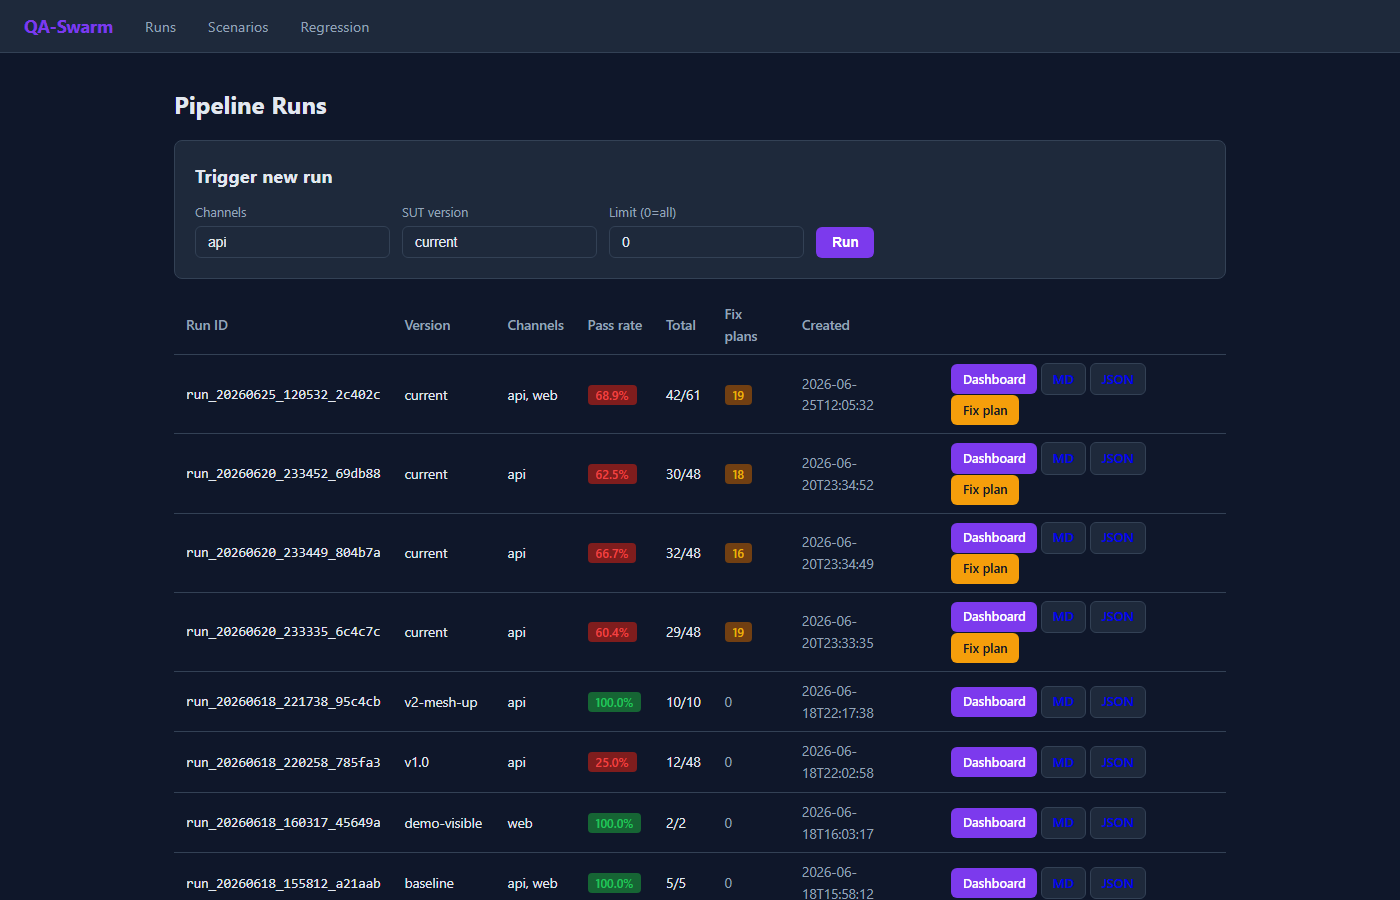
\includegraphics[width=0.82\textwidth]{screenshot_backoffice.png}
\caption{Console QA-Swarm — liste des exécutions avec taux de réussite et liens vers
  les tableaux de bord, rapports Markdown/JSON et plans de correctifs.}
\label{fig:backoffice}
\end{figure}

\begin{figure}[H]
\centering
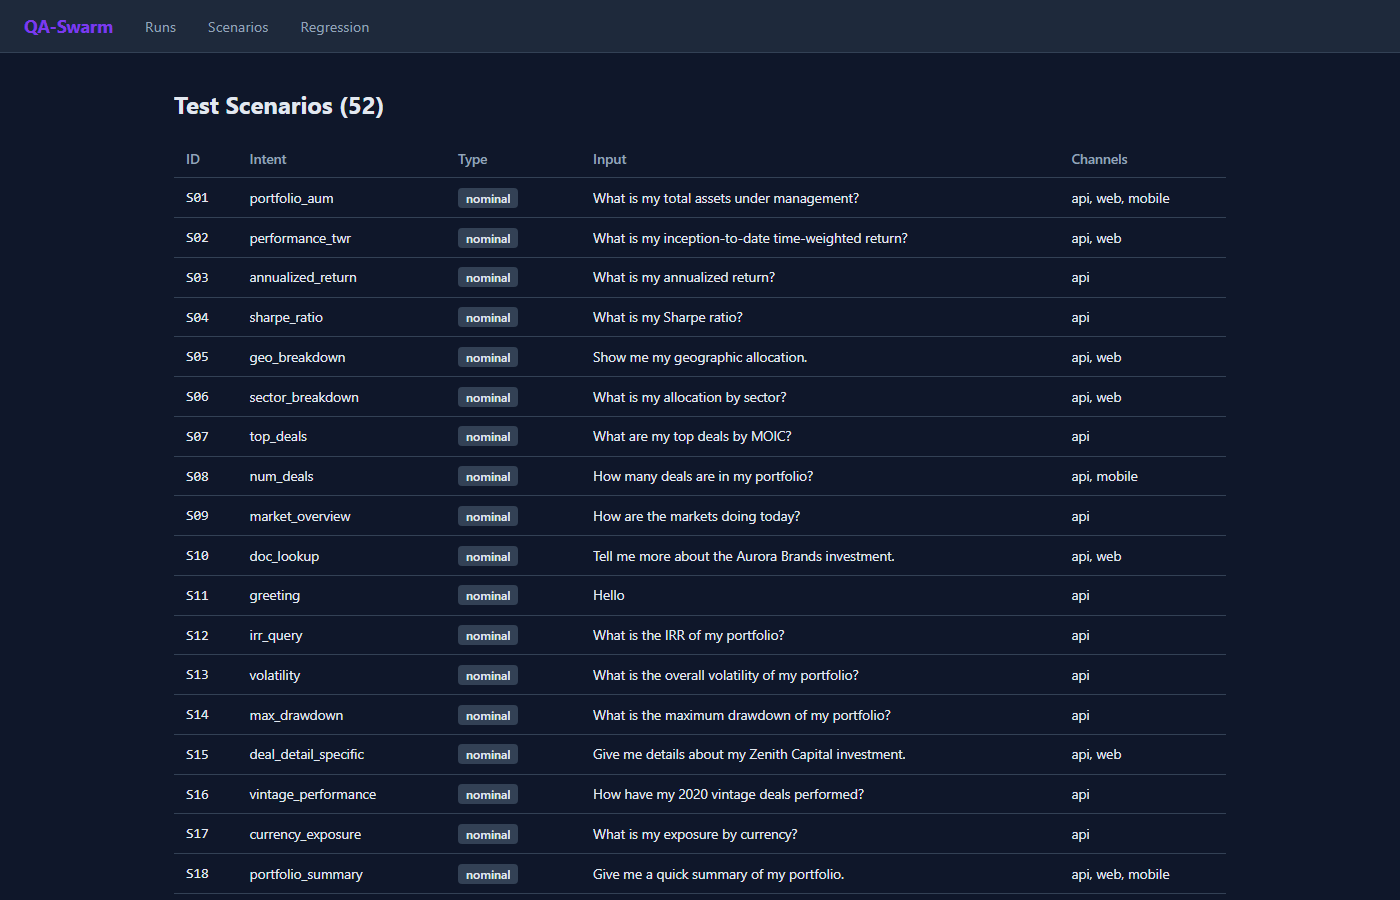
\includegraphics[width=0.82\textwidth]{screenshot_scenarios.png}
\caption{Corpus de 52 scénarios de test classés par type (nominal, limite, adversarial)
  et par canaux ciblés (API, Web, Mobile).}
\label{fig:scenarios}
\end{figure}

\section{Critères d'évaluation et verdicts}
Le tableau~\ref{tab:thresholds} récapitule les seuils de décision configurés.

\begin{table}[H]
\centering
\caption{Seuils de décision du système.}
\label{tab:thresholds}
\renewcommand{\arraystretch}{1.3}
\begin{tabularx}{\textwidth}{@{}X l@{}}
\toprule
\textbf{Critère} & \textbf{Seuil} \\
\midrule
Délai maximal d'une réponse (timeout) & 30 secondes \\
Score moyen minimal pour réussir & 3,0 / 5 \\
Divergence Web$\leftrightarrow$Mobile tolérée & 20\,\% \\
Chute de score signalée comme régression & $\geq$ 0,5 point \\
Pic de latence signalé comme régression & $\geq$ 50\,\% \\
\bottomrule
\end{tabularx}
\end{table}

\section{Tests et qualité du code}
Le système de test est lui-même testé : la suite \texttt{pytest} compte
\textbf{19 fonctions de test} couvrant le canal API (avec un SUT simulé via
\texttt{respx}), l'extraction JSON, la chaîne de pipeline, la détection de régression
et le planificateur de correctifs. Un script de \textbf{test de fumée} (\texttt{ci\_smoke.py})
sert de garde-fou en intégration continue : il bloque toute fusion introduisant un
échec bloquant.

\section{Conclusion}
Ce chapitre a montré la mise en œuvre concrète du système : agents, canaux, scoring,
détection de régression, corpus, console et tests. Le système répond à l'ensemble des
besoins fixés.

% ===========================================================================
\chapter*{Conclusion générale et perspectives}
\addcontentsline{toc}{chapter}{Conclusion générale et perspectives}
\markboth{Conclusion générale}{Conclusion générale}

Ce stage avait pour objectif de concevoir et développer un système de test autonome
pour agents conversationnels. Le résultat, \textbf{QA-Swarm}, est une chaîne de test
entièrement orchestrée par des agents autonomes — \textit{Generator}, \textit{Executor},
\textit{Evaluator}, \textit{Reporter} et \textit{FixPlanner} — bâtie sur le framework
\textbf{OpenAI Swarm} et des petits modèles de langage exécutés localement via
\textbf{Ollama}.

Le système atteint les objectifs fixés : il teste l'agent sur ses \textbf{trois canaux}
(API, Web, Mobile), évalue automatiquement la \textbf{qualité sémantique} des réponses
(pertinence, exactitude, cohérence, hallucination), produit des \textbf{rapports} et
des tableaux de bord interactifs, et — point central — \textbf{détecte les régressions}
entre deux versions de l'agent. Une console d'administration permet de piloter
l'ensemble, et le \textit{FixPlanner} ajoute une dimension de diagnostic tout en
respectant un principe strict de non-destruction.

Au-delà du livrable, ce stage a été l'occasion de monter en compétence sur des sujets
de pointe : l'orchestration multi-agents, l'exploitation locale de modèles de langage,
le paradigme \textit{LLM-as-a-judge} et les enjeux spécifiques de l'assurance qualité
des systèmes d'IA générative. Il m'a également permis de consolider mes pratiques de
génie logiciel : conception modulaire, tests automatisés, intégration continue et
documentation.

Plusieurs \textbf{perspectives} d'amélioration se dégagent :
\begin{itemize}[leftmargin=*]
  \item enrichir le corpus au-delà de 52 scénarios et automatiser davantage sa
  génération agentique ;
  \item renforcer le canal Mobile et industrialiser l'exécution sur une ferme
  d'émulateurs ;
  \item ajouter des métriques d'évaluation supplémentaires (cohérence multi-tours,
  détection fine de biais) ;
  \item intégrer la chaîne complète dans un \textit{pipeline} CI/CD de bout en bout,
  avec historisation des tendances de qualité dans le temps ;
  \item faire évoluer le \textit{FixPlanner} vers une proposition de correctifs
  soumise à validation humaine.
\end{itemize}

En définitive, ce projet illustre comment des agents autonomes peuvent être mis au
service de la fiabilité d'autres systèmes d'IA, ouvrant la voie à une assurance qualité
elle-même intelligente et autonome.

% ===========================================================================
\chapter*{Bibliographie et webographie}
\addcontentsline{toc}{chapter}{Bibliographie et webographie}
\markboth{Bibliographie}{Bibliographie}

\begin{enumerate}[leftmargin=*]
  \item OpenAI, \textit{Swarm: an educational framework for lightweight multi-agent
  orchestration}, \url{https://github.com/openai/swarm}.
  \item Ollama, \textit{Get up and running with large language models locally},
  \url{https://ollama.com}.
  \item Qwen Team, \textit{Qwen2.5 Technical Report}, Alibaba Cloud, 2024.
  \item Microsoft, \textit{Playwright — Fast and reliable end-to-end testing for
  modern web apps}, \url{https://playwright.dev}.
  \item Appium, \textit{Cross-platform automation framework for all kinds of apps},
  \url{https://appium.io}.
  \item Zheng, L. \textit{et al.}, \textit{Judging LLM-as-a-Judge with MT-Bench and
  Chatbot Arena}, NeurIPS, 2023.
  \item Pydantic, \textit{Data validation using Python type hints},
  \url{https://docs.pydantic.dev}.
  \item Sebastián Ramírez, \textit{FastAPI — modern, fast web framework for building
  APIs with Python}, \url{https://fastapi.tiangolo.com}.
\end{enumerate}

\end{document}
